
\begin{frame}{Modelling of Water Distribution Networks}
	\begin{itemize}
		\item General principles for modelling fast regime very similar to circuit analysis.
		\begin{itemize}
			\item Water flows = currents.
			\item Pressures = voltages.
			\item Network components behave similarly to circuit components, but resistors generally non-linear.
		\end{itemize}
		\item Graph theory is combined with physics-induced boundary conditions to yield model of fast regime.
	\end{itemize}
\end{frame}
% general installation instructions



\begin{frame}{Modelling of Water Distribution Networks}{Graph Theory}
	Graph theory describes a networked system as a directed graph composed of edges and vertices.
	
	\begin{figure}[h!]
		\centering
		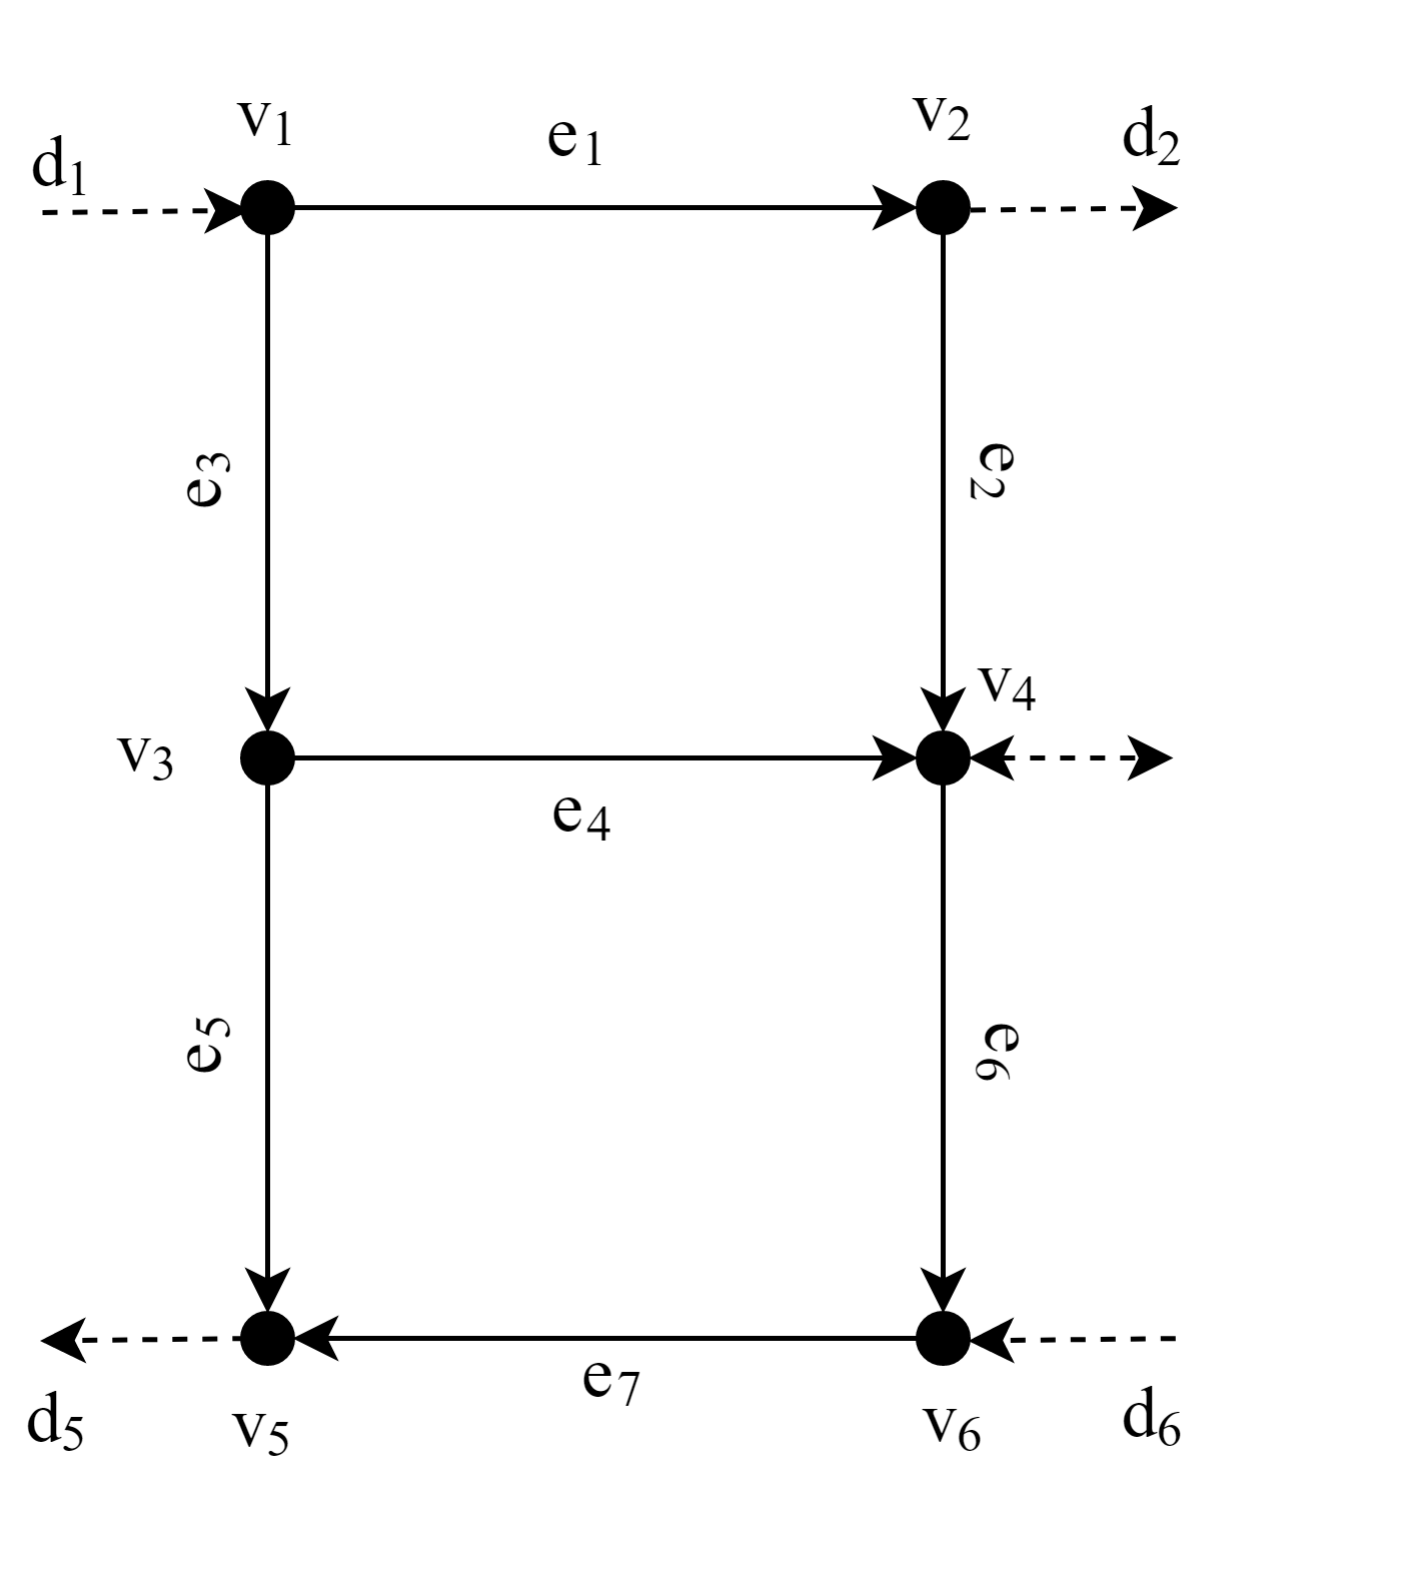
\includegraphics[width=0.4\textwidth]{Topics/SystemModel/Graphics/Graph.png}
		\caption{Graph of simplified WDN network. From \cite{Rathore930}.}
		\label{fig:graph}
	\end{figure}
	
\end{frame}


\begin{frame}{Modelling of Water Distribution Networks}{Incidence and Loop matrices}
Auxiliary matrices can be defined to mathematically describe the network:


\begin{equation*}
	\begin{aligned}
		&H_{i,j} = \begin{cases}
			1 & \text{If $j$th edge leaves $i$th node}\\
			-1 & \text{If $j$th edge enters $i$th node} \\
			0 & \text{If $j$th edge and $i$th node unconnected} 
		\end{cases} \\
		&B_{i,j} = \begin{cases}
			1 & \text{If direction of $ i $th loop and} \text{ $j$th edge agree}\\
			-1 & \text{If direction of $ i $th loop and} \text{ $j$th edge disagree}\\
			0 & \text{If $ i $th loop excludes $ j $th edge}\\
		\end{cases}
	\end{aligned}
\end{equation*}

\end{frame}


\begin{frame}{Modelling of Water Distribution Networks}{Incidence and Loop matrices: Example}
Example:

\begin{equation}
	H = \begin{bmatrix}
		1 & 0 & 1 & 0 & 0 & 0 & 0\\
		-1 & 1 & 0 & 0 & 0 & 0 & 0\\
		0 & 0 & -1 & 1 & 1 & 0 & 0\\
		0 & -1 & 0 & -1 & 0 & 1 & 0\\
		0 & 0 & 0 & 0 & -1 &  0  & -1\\
		0 & 0 & 0 & 0 & 0 & -1 & 1
	\end{bmatrix}
	\label{eq:H_simplified}
\end{equation} 

\begin{equation}
	\bar{H} = \begin{bmatrix}
		1 & 0 & 1 & 0 & 0 & 0 & 0\\
		-1 & 1 & 0 & 0 & 0 & 0 & 0\\
		0 & 0 & -1 & 1 & 1 & 0 & 0\\
		0 & -1 & 0 & -1 & 0 & 1 & 0\\
		0 & 0 & 0 & 0 & -1 &  0  & -1
		%0 & 0 & 0 & 0 & 0 & -1 & 1
	\end{bmatrix}
\end{equation}
\begin{equation}
	B = \begin{bmatrix}
		1 & 0 & 1 & -1 & -1 & 1 & 1\\
		0 & 1 & 0 & 0 & -1 & 1 & 1\\
	\end{bmatrix}
\end{equation}
\end{frame}


\begin{frame}{Modelling of Water Distribution Networks}{Demand Matrices}
Whether a node is open to atmosphere or not, or connected to a tank, can be described with matrices F and G respectively.
	
	
\begin{equation}
	F = \begin{bmatrix}
		1 & 0 & 0 & 0 \\
		0 & 1 & 0 & 0 \\
		0 & 0 & 0 & 0 \\
		0 & 0 & 0 & 0 \\
		0 & 0 & 1 & 0 & \\
		0 & 0 & 0 & 1 &
	\end{bmatrix}
	 , G = \begin{bmatrix}
		0  \\
		0  \\
		0  \\
		1  \\
		0 \\
		0 
\end{bmatrix}
\end{equation} 


	
\end{frame}



\begin{frame}{Modelling of Water Distribution Networks}{General Component Model}
	The edges of the WDN can be described with a pressure and flow relationship, analogous to the current and voltage of an electrical component. \\
	\medskip
	This project uses pipes, valves and pumps as edge components. \\
	\medskip
	The general relationship between pressure and flow can be defined as:
	
	\begin{equation}\label{eq:PressureFunction}
		\Delta p = \mathcal{J}\dot{q} + \lambda(q) + \mu(q, \Theta) + \alpha(q, \omega) -\Delta h
	\end{equation}
	
	
\end{frame}




\begin{frame}{Modelling of Water Distribution Networks}{Pipe model}
The pressure drop across a pipe is defined as:

	\begin{equation}
		\Delta{p_{k}} = \mathcal{J}\dot{q} + \lambda(q) + \Delta z
	\end{equation}

where:

	\begin{equation}
		\lambda_{k}(q_{k})  =	\Big(f \cdot \frac{8\cdot L\cdot q^{2}}{\pi^{2}\cdot g \cdot D^{5}} + k_{f}\cdot \frac{8\cdot q^{2}}{\pi^{2}\cdot g \cdot D^{4}}\Big)\cdot g \cdot \rho
	\end{equation}
	
	
	\begin{equation}
		\mathcal{J} = \frac{L\cdot \rho}{A}
	\end{equation}
	
	\begin{equation}
		\Delta{z_{k}} = \rho \cdot g \cdot \Delta{h_{k}}
	\end{equation}
\end{frame}



\begin{frame}{Modelling of Water Distribution Networks}{Valve model}
	The pressure drop across a valve is defined as:
	\begin{equation}\label{eq:ValvePressure}
		\Delta p_{k} = \mu(q,OD) = \frac{1}{K_{valve}(\Theta)^2} \cdot |q|\cdot q 
	\end{equation}
	
	where OD is the opening degree of the valve.\\
	
	Deriviation:
	
	\begin{equation}\label{eq:HydrodynamicRatio}
		\frac{\Delta p_1}{q_1^2} = \frac{\Delta p_2}{q_2^2} 	\Leftrightarrow
		q_1 = q_2\cdot\sqrt{\frac{\Delta p_1}{\Delta p_2}}
	\end{equation}
\begin{equation}\label{eq:Kvalve}
	q = q_n(\Theta)\cdot\sqrt{\frac{\Delta p_1}{1}} = K_{valve}(\Theta)\cdot\sqrt{\Delta p_1}
\end{equation}
\end{frame}


\begin{frame}{Modelling of Water Distribution Networks}{Pump model}
	The pressure drop across a pump is defined as:
	\begin{equation}\label{eq:PumpPressure}
		\Delta p_{k} =   a_0\cdot \omega^2 +  a_1\cdot \omega \cdot q -a_2\cdot |q|\cdot q
	\end{equation}
	
	where $[a_0,a_1,a_2]$ is a tuple of coefficients that describe the pump's characteristic curve, $q$ is the flow rate through the pump, and $\omega$ is the rotational velocity of the pump.
	
\end{frame}




\begin{frame}{Modelling of Water Distribution Networks}{Assumptions}
	Kirchhoff's node and mesh law:
	
	\begin{equation}
		Hq = d  
	\end{equation} 
	\begin{equation}
		B\Delta p = B H^T p = 0 \wedge B\Delta h = B H^T h = 0 
	\end{equation} 

	Mass conservation:
	\begin{equation}\label{eq:MassConservation}
		d_n = -\sum_{i=1}^{n-1}d_i
	\end{equation}
\end{frame}


\begin{frame}{Modelling of Water Distribution Networks}{Lemmas}
	Lemma 4.1:
	\begin{equation}\label{eq:TreePartitionLemma}
		H_T\bar{H}_T^{-1} = \begin{bmatrix} I_{n-1} \\ -\mathbf{1}^T	\end{bmatrix}
	\end{equation}
	where $\mathbf{1}$ is a vector of ones and $I_{n-1} \in \mathbb{R}^{n-1 \times n-1}$ is an identity matrix.


	Lemma 4.2:
	\begin{equation}\label{eq:EdgeFlowDecomposition}
		q = B^T q_C +
		\begin{bmatrix}
			0_{C \times n-1} \\ \bar{H}_T^{-1} 
		\end{bmatrix}
		\bar{d}
	\end{equation}

\end{frame}


\begin{frame}{Modelling of Water Distribution Networks}{System model}
	Non linear differential equation:
	\begin{equation}
		\Phi\mathcal{J}\Phi^T \dot{q} = -\Phi\Big(\lambda(q_n)+\mu(q_n)+\alpha(q_n)\Big) + \Psi(\bar{h}-\mathbf{1}h_0) + \mathcal{I}(p_{\tau}-\mathbf{1}p_0)
	\end{equation}

	Where the matrices $\Phi, \Psi, \mathcal{I}$ are defined as:
	
	\begin{equation}
		\Phi \triangleq 
		\begin{bmatrix} 
			I & -\bar{H}_C^T\bar{H}_T^{-T} \\ 0 & \bar{F}^T\bar{H}_T^{-T} \\ 0  & \bar{G}^T\bar{H}_T^{-T} \\ 
		\end{bmatrix}
		, \qquad
		\Psi \triangleq
		\begin{bmatrix}
			0 \\ \bar{F}^T \\ \bar{G}^T
		\end{bmatrix}
		, \qquad
		\mathcal{I} \triangleq
		\begin{bmatrix}
			0 \\ 0 \\ I
		\end{bmatrix}
	\end{equation}

	\begin{equation}
		\mathcal{P}: (\Phi \mathcal{J} \Phi^T)^{-1}
	\end{equation}
	
	
	
	\begin{equation}\label{eq:NonLinearModelSimplified}
		\begin{split}
			\dot{q}_n &=  -\mathcal{P}\Phi\Big(\lambda(q_n)+\mu(q_n)+\alpha(q_n)\Big) + \mathcal{P}\Big(\Psi(\bar{h}-\mathbf{1}h_0) + \mathcal{I}(p_{\tau}-\mathbf{1}p_0)\Big) 
		\end{split}	
	\end{equation}


\end{frame}


